\documentclass[12pt,a4paper, english]{article}
% \documentclass[12pt,a4paper]{article}
% portuguese
% \usepackage[portuguese]{babel}
\usepackage{babel}
\usepackage{blindtext}

%for embedding images
% \usepackage[pdftex]{graphicx}
% \usepackage[demo]{graphicx}
\usepackage{graphicx}
% para a cor do texto
\usepackage[usenames, dvipsnames]{color}

\usepackage{listings} 
%for proper url entries

\usepackage{url}
%for creating links in the pdf version and other additional pdf attributes, no effect on the printed document
% \usepackage[bookmarks, colorlinks=false, linkcolor=red, pdfborder={0 0 0}, pdftitle={Tese}, pdfauthor={Goncalo Silva Pereira - 2009111643}, pdfsubject={Evaluate the robusteness of Cloud}, pdfkeywords={Faults, Errors, Failures, Vulnerabilities, Fault Injection, Fault Tolerance, Security, Robustness}, linktoc=section, citecolor=green, filecolor=cyan, urlcolor=magenta, urlbordercolor={0 1 1}, citebordercolor={0 1 0}, linkbordercolor={1 0 0}]{hyperref} 
% \usepackage[bookmarks=true, pdftitle={Tese}, pdfauthor={Goncalo Silva Pereira - 2009111643}, pdfsubject={Evaluate the robusteness of Cloud}, pdfkeywords={Faults, Errors, Failures, Vulnerabilities, Fault Injection, Fault Tolerance, Security, Robustness}, linktoc=all]{hyperref}
\usepackage{hyperref}
\hypersetup{
	% bookmarks,
	pdftitle={Tese}
	,pdfauthor={Goncalo Silva Pereira - 2009111643}
	,pdfsubject={Evaluate the robustness of Cloud}
	,pdfkeywords={Faults, Errors, Failures, Vulnerabilities, Fault Injection, Fault Tolerance, Security, Robustness}
	,linktoc=all
} 

% to go to the begin of figures
\usepackage{caption}
% \usepackage[all]{hypcap}

\usepackage{bookmark}

% indent first paragraph
\usepackage{indentfirst}
%\usepackage[final]{pdfpages} %for embedding another pdf, remove if not required

% package to use acronyms
\usepackage{acro}
%!TEX root = main.tex

% class `abbrev': abbreviations:
\DeclareAcronym{api}{
  short = API ,
  long  = Application Programming Interface ,
  class = abbrev
}
\DeclareAcronym{cots}{
  short = COTS ,
  long  = Components of the shelf ,
  class = abbrev
}
\DeclareAcronym{dos}{
  short = DOS ,
  long  = Denial of Service ,
  class = abbrev
}
\DeclareAcronym{ddos}{
  short = DDOS ,
  long  = Distributed Denial of Service ,
  class = abbrev
}
\DeclareAcronym{fo}{
  short = FO ,
  long  = Fail-Operational ,
  class = abbrev
}
\DeclareAcronym{fs}{
  short = FS ,
  long  = Fail-Safe ,
  class = abbrev
}
\DeclareAcronym{g-swfit}{
  short = G-SWFIT ,
  long  = Generic Software Fault Injection Technique ,
  class = abbrev
}
\DeclareAcronym{iaas}{
  short = IaaS ,
  long  = Infrastructure-as-a-Service ,
  class = abbrev
}
\DeclareAcronym{iso}{
  short = ISO ,
  long  = International Organization for Standardization ,
  class = abbrev
}
\DeclareAcronym{odc}{
  short = ODC ,
  long  = Orthogonal Defect Classification ,
  class = abbrev
}
\DeclareAcronym{qos}{
  short = QOS ,
  long  = Quality-of-Service ,
  class = abbrev
}
\DeclareAcronym{ots}{
  short = OTS ,
  long  = Off-the-shelf ,
  class = abbrev
}
\DeclareAcronym{paas}{
  short = PaaS ,
  long  = Platform-as-a-Service ,
  class = abbrev
}
\DeclareAcronym{saas}{
  short = SaaS ,
  long  = Software-as-a-Service ,
  class = abbrev
}
\DeclareAcronym{swifi}{
  short = SWIFI ,
  long  = Software Implemented Fault Injection ,
  class = abbrev
}
\DeclareAcronym{odc}{
  short = ODC ,
  long  = Orthogonal Defect Classification ,
  class = abbrev
}

% add notes to margins
\usepackage{marginnote}
% \usepackage[top=1cm, bottom=1cm, outer=0.5cm, inner=0.5cm, heightrounded, marginparwidth=1cm, marginparsep=1cm]{geometry}
\usepackage[utf8]{inputenc}

% append another pdfs
\usepackage{pdfpages}

% to use landscape mode
\usepackage{lscape}
	
% \usepackage[export]{adjustbox}

% \usepackage[portrait]{gmeometric} 

\newcommand*{\red}{\textcolor{red}}

% edit footer and header
\usepackage{fancyhdr}
\pagestyle{fancy}
\fancyhf{} % sets both header and footer to nothing
\renewcommand{\headrulewidth}{0pt}
% your new footer definitions here
\cfoot{\hyperref[toc]{\thepage}}
% \fancyhead[L]{}
% \renewcommand{\headrulewidth}{0pt}


% % to reduce font size of table of contents
% % THESE COUPLE LINES ARE THAT YOU NEED FOR THE 2ND PART
% \AtBeginDocument{
%   \addtocontents{toc}{\tiny}
%   \addtocontents{lof}{\tiny}
% }
% % THESE COUPLE LINES ARE THAT YOU NEED FOR THE 1ST PART
% \usepackage{xpatch}
% \makeatletter
% \xpatchcmd{\tableofcontents}{\contentsname \@mkboth}{\small\contentsname \@mkboth}{}{}
% \xpatchcmd{\listoffigures}{\chapter *{\listfigurename }}{\chapter *{\small\listfigurename }}{}{}
% \makeatother


% view frame in page, arround all areas, page, footer, header
% \usepackage{showframe}

% to put title, author and data in begin of thesis and use it
% \usepackage{authoraftertitle}
% \title{Evaluate the robusteness of Cloud coisas}
% \author{Gonçalo Silva Pereira}
% \date{\today}

% block quote with big quotation marks 
\usepackage[T1]{fontenc}
\usepackage{libertine}
\usepackage{graphicx}
\usepackage{framed}

\newcommand*\openquote{\makebox(25,-22){\scalebox{5}{``}}}
\newcommand*\closequote{\makebox(25,-22){\scalebox{5}{''}}}
% \definecolor{BlueLUH}{cmyk}{1.0,0.7,0,0}
\definecolor{BlueLUH}{cmyk}{0.0,0.0,0,0}
% sombreado
\colorlet{shadecolor}{BlueLUH!80!black!20}
% branco
\colorlet{shadecolor}{BlueLUH!0!black!0}

\makeatletter
\newif\if@right
\def\shadequote{\@righttrue\shadequote@i}
\def\shadequote@i{\begin{snugshade}\begin{quote}\openquote}
\def\endshadequote{%
  \if@right\hfill\fi\closequote\end{quote}\end{snugshade}}
\@namedef{shadequote*}{\@rightfalse\shadequote@i}
\@namedef{endshadequote*}{\endshadequote}
% end block quote

\begin{document}
%!TEX root = main.tex
\begin{titlepage}

\begin{center}

\begin{figure}[!ht]
\begin{center}

\includegraphics[width=0.5\textwidth]{img/uc.jpg}
% \includegraphics[width=1\textwidth]{img/fctuc.jpg}
% \nocaption
\end{center}
\end{figure}
\vspace{0.9cm}
% \textup{\small {\bf Thesis}}\\[0.3in]
% \textup{\small {\bf Estágio}}\\[0.3in]

\small{\bf MSc in Informatics Engineering}\\[0.3in]
\small{\bf Entermediate Report}\\[0.7in]
% \small{\bf Mestrado em Engenharia Informática}\\[1.3in]

% Title
\Large
% \textbf {Relatório de estágio}\\[0.2in]
% \textbf{Avaliação da Robustez de Plataformas Cloud}\\[1.5in]
\textbf{Evaluate the robustness of Cloud}\\[0.9in]

% team
\Large{Gonçalo Silva Pereira}\\
\vspace{0.5cm}

\normalsize
\begin{table}[h]
\centering
\begin{tabular}{lr}\hline
Supervisor     &  Raul Barbosa\\
Co-Supervisor  &  Henrique Madeira\\ \hline
% Juri Arguente  &  Filipe Araujo\\
% Juri Vogal	   &  Antonio Jorge Silva Cardoso\\ \hline
\end{tabular}
\end{table}

% Bottom of the page
\vspace{3cm}
\Large{Department of Informatics Engineering}\\
\normalsize
\textsc{University of Coimbra}
% Faculdade de Ciências e Tecnologia\\
\vspace{0.2cm}\\


\dateenglish
\today

\end{center}
\end{titlepage}


%!TEX root = main.tex

% supress page number
% \pagenumbering{gobble}

% \maketitle

% include other pages
%!TEX root = main.tex

% \section*{Dedication}
% \addcontentsline{toc}{section}{Dedication}
\pagestyle{empty}
\begin{center}

\emph{Dedication}

\end{center}



\newpage
\pagestyle{fancy}
\section*{Acknowledgements}
% \addcontentsline{toc}{section}{Acknowledgments}

I would like to thank to ------ and to professors Raul Barbosa and Henrique Madeira, who are role models, by their support and help to take good decisions.\\

Thank my girlfriend for her support, understanding and the fellowship along this path. At my friends and colleagues of Department of Informatics Engineering the patience, support and for all times they have given me. \\

Last but certainly not least, I would like to thank my family for encouragement, love and all the unconditional and constant support that led me to fulfill this dream. Obrigado!\\

% \hfill Obrigado! \\

% \hfill Gonçalo Silva Pereira

% \vspace{4cm}
\emph{\hfill Gonçalo Silva Pereira}

\clearpage

% \section{Software Quotes}
\vspace*{\fill}
\pagestyle{empty}
% \addcontentsline{toc}{section}{Software Quotes}

% http://www.devtopics.com/101-more-great-computer-quotes/
\begin{shadequote}
Bridges are normally built on-time, on-budget, and do not
fall down. On the other hand, software never comes in on-time
or on-budget. In addition, it always breaks down.\par\emph{Alfred Z. Spector, Google Research}
\end{shadequote}

\begin{shadequote}
"I have no special talents. I am only passionately curious." \par\emph{Albert Einstein}
\end{shadequote}


% \begin{shadequote}
% The computer was born to solve problems that did not exist before.\par\emph{Bill Gates}
% \end{shadequote}

% \begin{shadequote}
% Tell me and I forget.
% Teach me and I remember.
% Involve me and I learn.\par\emph{Benjamin Franklin}
% \end{shadequote}

% \begin{shadequote}
% Once you get a B.S. in Computer Science,
% you think you know everything. Once you get an M.S.,
% you realise no one knows anything!.\par\emph{Unknown}
% \end{shadequote}
\clearpage
\pagestyle{fancy}

\pagenumbering{roman}

\setcounter{tocdepth}{2}
\renewcommand{\baselinestretch}{0.9}\normalsize
\pdfbookmark{\contentsname}{toc}
\tableofcontents \label{toc}
% \addcontentsline{toc}{section}{Contents}
% \renewcommand{\baselinestretch}{1.0}\normalsize
\newpage

\listoffigures
\listoftables

\clearpage
\printacronyms[include-classes=abbrev,name={\subsection*{Abbreviations}}]
% \printacronyms[include-classes=abbrev,name=Abbreviations]
% \addcontentsline{toc}{section}{Abbreviations}

% glossary
% \glsaddall
% \printglossaries
\clearpage
%!TEX root = main.tex
\clearpage
\pagenumbering{arabic}

\addcontentsline{toc}{section}{Abstract}

\begin{abstract}
The Cloud Computing is a new paradigm that provides on demand self-service resources, broad network access, resource pooling, rapid elasticity and a measured service through four different models, community, hybrid, private and public.

The main objective of this paradigm is to allow users to get the most of the technology without having the knowledge and skills to ensure the proper functioning of all the technologies involved, allowing the users to focus on their core business, rather than be blocked due to technological difficulties.

The fact of the virtualization being the fundamental technology that powers cloud computing, provide the reduction of IT cost while increase the efficiency, utilization and flexibility of their existing computer hardware.

However, the Cloud Computing is not free of external disturbance like security attacks, power surges, workload faults, hardware and software faults. Due to this reason, the theme of my dissertation is ``Evaluate the robustness of the Cloud'' and it is based on the development of a fault injector software, to, as the name suggests, inject faults into the software to test it in the cloud later. After the testing, the collected results will be evaluated using the CRASH Scale.\\



% \iftoggle{long}{\orange{O abstract começa com um âmbito demasiado abrangente, e até um pouco fora do tema principal da tese. Tem de ser re-escrito para ficar mais focado.}}


% \iftoggle{long}{\red{Breve contextualixação antes de dizer objetivo!!!
% \red{This thesis/dissertation presents an ????}}


% Nowadays, the Information and Communication Technologies are responsible for 2-4\% of CO\textsuperscript{2} emissions, but in the next five or ten years these will increase to 10\% \cite{wolter2012resilience}. Because of this, the next challenge is to reduce the costs of ICT and its impact in the environment while the IC services keep growing.


% Cloud computing is a new paradigm that provides on-demand self-service resources (computing, network and storage). It also promises to reduce the costs of ICT, but isn't free of external disturbance like security attacks, power surges, workload faults and others.

% Therefore, the theme of my dissertation is ``Evaluate the robustness of the Cloud''. I will design and implement a fault injector for software coded in C to evaluate the capacity of the cloud to recover from faults.\\
% }


\textbf{Keywords:} Robustness, Cloud Computing, Faults, Errors, Failures, Vulnerabilities, Fault Injection, Fault Tolerance.

\end{abstract}

%!TEX root = main.tex
\newpage
% \chapter{Introduction}
\section{Introduction}

\iftoggle{long}{\red{In the next subsections will be introduced the context and the scope of this project.}
\orange{1,2 ou 3 paragrafos descritivos do problema}}

\subsection{Contextualization}
\iftoggle{long}{\orange{Logo aqui deve ficar claro que os bugs existem, vão sempre existir, e que testar a capacidade de qualquer sistema crítico para lidar com bugs existentes é fundamental. Daí todo o trabalho. Não é claro por que razão (ou razões) isto é específico para a Cloud. Não é igual fazer-se para a Cloud ou para programas stand-alone clássicos?}}


The present dissertation describes the work developed in the scope of Master of Science in Informatics Engineering. It is focused on ``Evaluate the robustness of Cloud'' and this is a very important issue nowadays, because of the increasing usage of this.
It's characterized by the placement of data and software on remote infrastructure. Despite the numerous benefits, the reliability of these platforms hasn't kept the needs, and users trust on their applications to systems outside of personal control.

In this context, the problem of confidence in the entity that manages the platform where applications have been executed arises naturally. Any organization that put an application in the cloud (for example, Microsoft Azure or Amazon EC2) so should accept the assurances given by the service provider.

\iftoggle{long}{\red{This internship deals with the challenge of assessing the robustness of cloud platforms. The computing service provider uses virtualization to manage and allocate computing power to meet present needs of the application.}}


\iftoggle{long}{\red{Although, there are solid virtualization platforms, fault tolerance is still a research problem.}}


\iftoggle{long}{\red{resilience}}


\subsection{The project}

This project is based mainly in inject software faults. It was decided since there are already other people involved in the part of hardware faults.

\subsection{Objectives}

The main objective of this work is to evaluate the robustness of the cloud. To do that, I will design and implement a tool to inject software faults in source code of some applications.

Nevertheless, this objective is divided in some other goals:

\iftoggle{long}{\orange{Esta parte está bem, mas o passo de “evaluate the robustness of the cloud” para estes 3 objetivos é demasiado grande. Deve explicar-se um pouco mais, partindo de um objetivo grande, e progressivamente estabelecer o que aqui se chama “goals”.}}

\begin{itemize}
	\item Implement the thirteen operators specified by João Durães;
	\item Use the fault injector to emulate faults in applications, running in the cloud;
	\item Measure the time and the value obtained after running the app, in a normal scenario;
	\item Inject a fault in application, measure the time and the value after running the app;
	\item Compare the time and value in a normal scenario and in a scenario with faults;
	\item

	\item Generate derivations of main code of selected programs;
	\item Verify and analyze the effect of produced faults;
	\item Compile the programs with injected faults, by using make file.
\end{itemize}


\subsection{Document Structure}

In this document are specified all the related subjects with the project.

The second section presents the state-of-the-art in the related areas with particular emphasis to Cloud Computing and Fault Injection.

The third section is an important section of this report, because of the research involved in the execution of this work. It was necessary to take some important decisions based in research results, knowledge and my own experience.

The fourth section describes the work that has been done in Fault Injector, and the work that should be done in the next semester.

The fifth section explains other modules that need to be executed in this project to observe and evaluate the results of the fault injector.

In the last section, I will do an overview analyses of my work, in general the operators and the constraints developed. I will also talk about the work to be done in the next semester.


%!TEX root = main.tex
% \newpage
\subsection{Management}

\iftoggle{long}{\red{In this section is described the planning of work developed in this dissertation.}}

\subsubsection{Meetings}
About the meetings, the supervisor Raul Barbosa and I agreed that meeting once every week was the best option. Moreover they happened, with one or another change of schedule to reconcile with the other activities from both. In addition, I attended some general meetings of the project. In them, we could discuss concepts and the direction of the project with colleagues and teachers, among them: Raul Barbosa (supervisor), Henrique Madeira (co-supervisor), João Durães and João André Ferro.

\subsubsection{Risks}

As any other projects, this project have risks too.
% Risks related to the planning and execution of this dissertation.
Some of the risks are related to equipment failure and data lost and to prevent that this happen I use \textit{Github} to backup the source developed to the project and this report. This backups are done in all days that I do some improvements to this project.

The particularity of this project be in investigation nowadays, bring other risk to this project, associated to the publication of similar research, to reduce this risk, I will check with regularity electronic publications, and if similar research was published, I will modify the project to assure that adds value and it's not just like any other.

Moreover, I can have personal issues interfering with the progress of this project or lose the interest, and to prevent this I have selected a motivating topic at the beginning and I talk to the supervisor always that I have doubts.

This risks, the preventative measures and the recovery measures can be seen, in other perspective, at Appendix \ref{App:B}.

\subsubsection{Planning and Tracking}
In Appendix \ref{App:A}, is showed the Gantt diagram with the tasks that have been done during the first semester.
%  to first and to second semester.I'm not showing here the planned Gantt
As I postponed this dissertation for six months so, the scope and the context have changed. Now the two Gantt diagrams are incomparable.


%I have prioritized the tasks using the nomenclature in Table \ref{tab:classRequirements}:
%\begin{table}[!ht]
%\begin{tabular}{cc}
%\hline
%\textbf{Classification}                & \textbf{Mean}                                                                                                                                                           \\ \hline
%\multicolumn{1}{|c|}{\textit{Must}}    & \multicolumn{1}{c|}{\begin{tabular}[c]{@{}c@{}}Must be implement at project finish,\\  and his implementation is priority.\end{tabular}}                                \\ \hline
%\multicolumn{1}{|c|}{\textit{Nice}}    & \multicolumn{1}{c|}{\begin{tabular}[c]{@{}c@{}}May be part of the functionality implemented\\  at the end of project, and his implementation is optional.\end{tabular}} \\ \hline
%\multicolumn{1}{|c|}{\textit{Wishful}} & \multicolumn{1}{c|}{\begin{tabular}[c]{@{}c@{}}It's specified but his implementation is \\not expected until the end of project.\end{tabular}}                          \\ \hline
%\end{tabular}
%\caption {Classification of requirements} \label{tab:classRequirements}
%\end{table}

% \newpage
\iftoggle{long}{\red{About the development of this project, I have used an \emph{Agile Life Cycle} based in an \emph{Incremental Model}.}}

\iftoggle{long}{\red{porque? ajuda? com que objectivo? foi uma boa opção? quais eram as alternativas? em que falhavam? porque nao foram escolhidas? }}

\iftoggle{long}{\red{What are the requirements of this project???}}


%!TEX root = main.tex
\newpage
\section{State of the Art}

Nowadays, people use lot's of services based in cloud and lot's of companies choose to use them too. Using it, companies reduce the costs of IT infrastructure and people don't buy ``physical storage'' and don't care where are the data. The cloud service provide that the data is secure.
But, like any system, the cloud have problems such as another computer systems, software and hardware faults. And the resilience of the cloud is an important characteristic.

The increased use of cloud is related with a low usage of many dedicated servers, lower voltage levels, reduce noise margins and increase clock rates \cite{wolter2012resilience}.

The cloud providers offers resources ready to deliver \cite{wolter2012resilience}.

With this work, I want to inject software faults and analyze how the system react to them.

A lot of studies show that the software faults\cite{avizzienisbasic} it's the main cause of computer failures.

%In this work
%deliberate how

About 44\% of the software faults cannot be emulated \cite{madeira2000emulation}.

% \marginnote{especificar as abreviaturas...}[0cm]
% \ac{cots}
% \ac{g-swfit}
% \ac{odc}
% \ac{swifi}

I had access to the application of Robert Natella, called SAFE, that inject software faults, as I also have to do.

\subsection{SAFE - Robert Natella}
Safe is an application to inject faults in code written in C. This tool uses MCPP as parser, to get the tree of code. After that, write some .c files, variations of original files with operators applied. Robert Natella implemented thirteen operators in SAFE, same as João Durães\cite{duraes2006emulation}, but with the difference that Robert implemented at source code level, and João at binary level.



\newpage
\section{Research objectives and approach method}

\subsection{GCC Parser vs CDT Parser vs Bison}


\subsection{Cloud Computing}

Three levels of Cloud Computing:

\begin{itemize}
	\item \ac{iaas};
	\item \ac{paas};
	\item \ac{saas}.
\end{itemize}

The cloud computing isn't free of external disturbances\cite{wolter2012resilience}, the most importants are:
\begin{itemize}
 	\item Security attacks;
 	\item Accidents;
 	\item Power surges;
 	\item Workload faults;
 	\item Malfunction;
 	\item Worms
 	\item \ac{ddos} attacks.
 \end{itemize}

\subsection{Applications to inject faults}

\newpage
\section{Current work and preliminary results}

\newpage
\section{Work plan and implications}

Built three separated modules:

\begin{itemize}
	\item Generate the derivations of main code of selected programs;
	\item Verify and analyze the effect of produced faults;
	\item Compile the programs with injected faults, by using make file.
\end{itemize}

\subsection{Generate derivations}

I chose to use the most representative faults \cite{duraes2006emulation}, divided into missing, wrong and extraneous, specified individually further down:

\subsection{Contraints}

The contraints defined below was specified by João Durães in ... .

\begin{table}[h]
\begin{tabular}{|c|l|}
\hline
\textbf{Constraints}            & \multicolumn{1}{c|}{\textbf{Description}}                                     \\ \hline
\textbf{C01}       \label{C01}  & Return value of the function must not being used                              \\ \hline
\textbf{C02}       \label{C02}  & Call must not be the only statement in the block                              \\ \hline
\textbf{C03}       \label{C03}  & Variable must be inside stack frame                                           \\ \hline
\textbf{C04}       \label{C04}  & Must be the first assignment for that variable in the module                  \\ \hline
\textbf{C05}       \label{C05}  & Assignment must not be inside a loop                                          \\ \hline
\textbf{C06}       \label{C06}  & Assignment must not be part of a for construct                                \\ \hline
\textbf{C07}       \label{C07}  & Must not be the first assignment for that variable in the module              \\ \hline
\textbf{C08}       \label{C08}  & The if construct must not be associated to an else construct                  \\ \hline
\textbf{C09}       \label{C09}  & Statements must not include more than five statemens and not include loops    \\ \hline
\textbf{C10}       \label{C010} & Statements are in the same block, do not include more than 5 stats. not loops \\ \hline
\textbf{C11}       \label{C011} & There must be at leat two variables in this module                            \\ \hline
\end{tabular}
\end{table}

\subsubsection{Fault Types - Missing:}
\begin{itemize}
	\item \textbf{MIFS} - if construct plus statements

	This operator is based in the remotion of one conditional if. To do that, I need to verify the constraints c02, c08 and c09.

% \begin{table}[h]
% \begin{tabular}{ll}
% Constraints & Description                                                                 \\
% C02         & The if construct must not be the only statement in block                    \\
% C08         & The if construct must not be associated to an else construct                \\
% C09         & Statements must not include more than five statements and not include loops
% \end{tabular}
% \end{table}

	\item \textbf{MLAC} - AND sub-expr in expression used as branch condition
	\item \textbf{MFC}  - function call
	\item \textbf{MIA}  - if construct around statements
	\item \textbf{MLOC} - OR sub-expr in expression used as branch condition
	\item \textbf{MLPA} - small and localized part of the algorithm
	\item \textbf{MVAE} - variable assignment using an expression
	\item \textbf{MFCT} - functionality
	\item \textbf{MVAV} - variable assignment using an value
	\item \textbf{MIEB} - if construct plus statements plus else before statements
	\item \textbf{MVIV} - variable initialization
\end{itemize}

\subsubsection{Fault Types - Wrong:}
\begin{itemize}
	\item \textbf{WLEC} - logical expression used as branch condition
	\item \textbf{WALL} - algorithm - large modifications
	\item \textbf{WVAV} - value assigned to variable
	\item \textbf{WAEP} - arithmetic expression in parameter of function call
	\item \textbf{WSUT} - data types or conversion used
	\item \textbf{WPFV} - variable used in parameter of function call
\end{itemize}

\subsubsection{Fault Types - Extraneous:}
\begin{itemize}
	\item \textbf{EVAV} - variable assignment using another variable
\end{itemize}


\subsection{Analyze the effects}

The fault injected results is equal to the real software faults?

\subsection{Compile programs}

Select five to ten programs to test.


%!TEX root = main.tex
\clearpage
\section{Conclusion}

\subsection{Global vision}

In table \ref{tab:operators_status}, it's possible to view at \green{green color}, the operators that were implemented in the first semester of this dissertation. As can be seen, I have implemented five of thirteen operators that João Durães specified. The first operator that I have implemented with success was the \ac{mifs}, and as the operators \ac{mia} and \ac{mieb} are similar and have some constraints in common, then I implemented them.

% \clearpage
% \begin{table}[ht]
% \begin{tabular}{c}
% 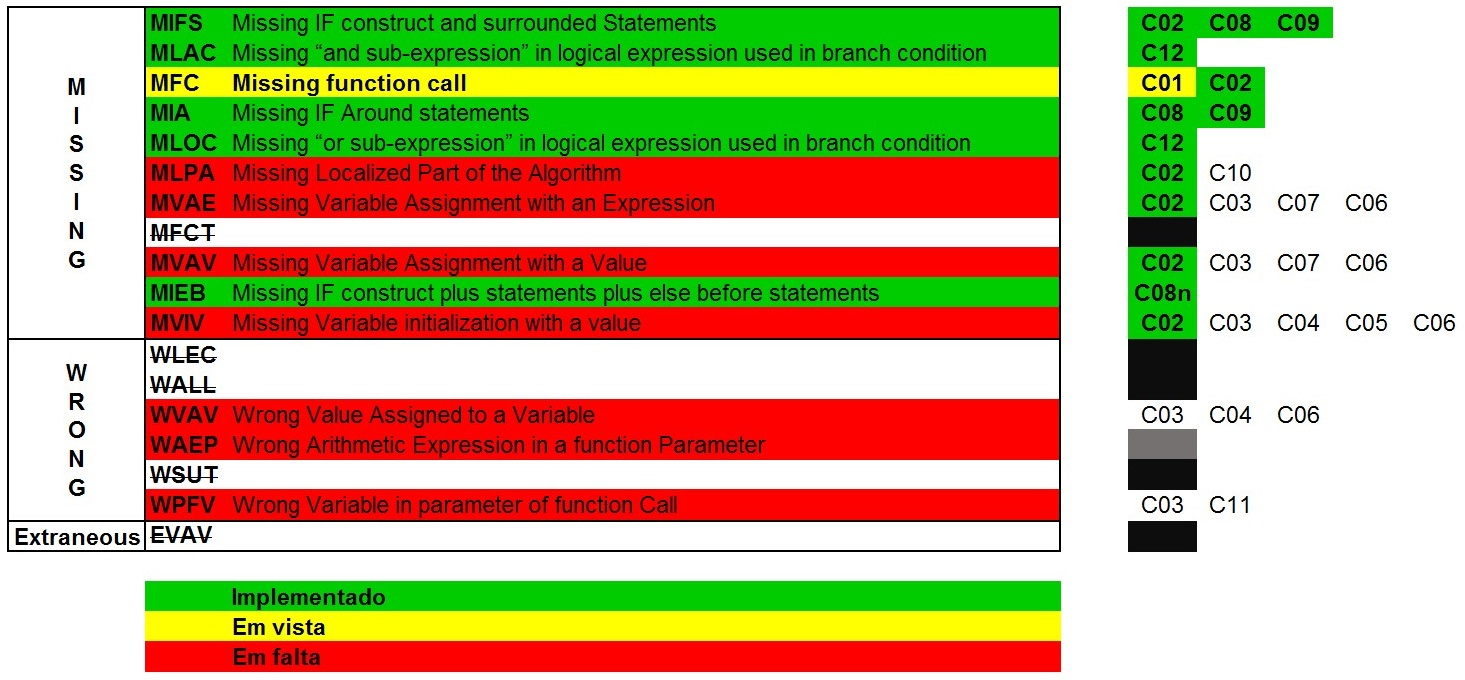
\includegraphics[width=1.1\textwidth]{img/operators_status.jpg}
% \end{tabular}
% \caption{\small \sl State of the operators and its constraints.\label{tab:operators_status}}
% \end{table}


\begin{table}[!ht]
\begin{tabular}{|l|p{12cm}|}
\hline
\textbf{Fault Type}		& \multicolumn{1}{c|}{\textbf{Description}}		\\ \hline \hline
MFC        				& \Acl{mfc}  									\\ \hline
\green{MIA}        		& \green{\Acl{mia}} 							\\ \hline
\green{MIEB}       		& \green{\Acl{mieb}} 							\\ \hline
\green{MIFS}       		& \green{\Acl{mifs}} 							\\ \hline
\green{MLAC}       		& \green{\Acl{mlac}} 							\\ \hline
\green{MLOC}       		& \green{\Acl{mloc}} 							\\ \hline
MLPA       				& \Acl{mlpa} 									\\ \hline
MVAE       				& \Acl{mvae} 									\\ \hline
MVAV       				& \Acl{mvav} 									\\ \hline
MVIV       				& \Acl{mviv} 									\\ \hline
WAEP       				& \Acl{waep} 									\\ \hline
WPFV       				& \Acl{wpfv} 									\\ \hline
WVAV       				& \Acl{wvav} 									\\ \hline
\end{tabular}
\caption{\small \sl State of the operators.\label{tab:operators_status}}
\end{table}

In table \ref{tab:constraints_status}, is also possible to check that I have implemented three of eleven constraints related to the thirteen operators, represented at \green{green color}.

\begin{table}[!ht]
\centering
\begin{tabular}{|c|p{12cm}|}
\hline
\textbf{Constraints}            & \multicolumn{1}{c|}{\textbf{Description}}                                     \\ \hline \hline
\textbf{C01}         & \Acl{c01} \\ \hline
\green{\textbf{C02}} & \green{\Acl{c02}} \\ \hline
\textbf{C03}         & \Acl{c03} \\ \hline
\textbf{C04}         & \Acl{c04} \\ \hline
\textbf{C05}         & \Acl{c05} \\ \hline
\textbf{C06}         & \Acl{c06} \\ \hline
\textbf{C07}         & \Acl{c07} \\ \hline
\green{\textbf{C08}} & \green{\Acl{c08}} \\ \hline
\green{\textbf{C09}} & \green{\Acl{c09}} \\ \hline
\textbf{C10}         & \Acl{c10} \\ \hline
\textbf{C11}         & \Acl{c11} \\ \hline
\end{tabular}
\caption{\small \sl State of the constraints.\label{tab:constraints_status}}
\end{table}

\begin{table}[!ht]
\centering
\begin{tabular}{|c|p{12cm}|}
\hline
\textbf{Constraints}            & \multicolumn{1}{c|}{\textbf{Description}}                                     \\ \hline \hline
\green{\textbf{C08n}}         & \green{\Acl{c08n}} \\ \hline
\green{\textbf{C12}}          & \green{\Acl{c12}} \\ \hline
\end{tabular}
\caption{\small \sl State of the other constraints.\label{tab:otherConstraints_status}}
\end{table}

% \iftoggle{long}{\red{version number}}
\break
Below, in the figure \ref{tab:version} can be seen the numbering system of versions of fault injector. The ``b'' represents that are implemented two constraints which isn't specified by João Durães. For example, if I implement three, then will be ``c'', and so on. The current version of the injector also has five operators and three constraints implemented, from those specified by João Durães. When the version numbering achieves 0.13.11 then the injector will be in the version number one.

\begin{figure}[!ht]
\begin{center}
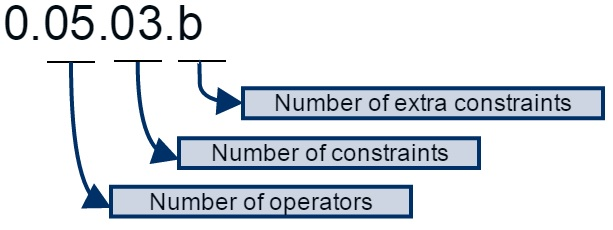
\includegraphics[width=0.6\textwidth]{version.jpg}
\caption{\small \sl Version number.\label{tab:version}}
\end{center}
\end{figure}

\clearpage
\subsection{Future work and experiments}

In the future, I have planned to implement the other operators and constraints. I will use regression testing to verify if when I coded one new operator or constraint I didn't mess with the operators and constraints previous implemented.
In addition, I will add to the fault injector a user interface, to turn this software more user-friendly, and a name.

Furthermore, in the next semester, I will study the hypervisor and I will implement some scenarios to evaluate the behavior of the cloud with and without faults.



% \textit{``The purpose of regression testing is to ensure that changes made to software, such as adding new features or modifying existing features, have not adversely affected features of the software that should not change. Regression testing is usually performed by running some, or all, of the test cases created to test modifications in previous versions of the software.''}
% \red{From version to version, I use a regression testing to test the fault injector to guarantee that application doesn't regarded.}

\iftoggle{long}{\orange{Mais do que “future work” é necessário um plano para o segundo semestre, relativamente detalhado.}}


% \iftoggle{long}{\orange{Globalmente há várias coisas que não estão suficientemente bem explicadas:}}


\iftoggle{long}{\orange{- exatamente quais são as características novas da cloud, que devem ser avaliadas por injeção de falhas (podemos conversar sobre isto)}}


% \iftoggle{long}{\orange{- qual a razão para se desenvolver algo novo, quando a ferramenta do Natella já faz muito (lembro-me que colecionámos muitos argumentos que estão anotados)}}


% \iftoggle{long}{\orange{- como é que se vai dar uso ao que está implementado? far-se-ão experiências, os resultados serão classificados e analisados certamente}}


% \iftoggle{long}{\orange{- o estado da arte deveria ponderar os prós e os contras de todas as técnicas para injeção de falhas de software (binário, instrumentação, source code, runtime, etc.)}}


% \iftoggle{long}{\orange{- o texto deve ser clarificado, mas essencialmente é no plano das ideias que muitas vezes está pouco claro: por que razão se está a fazer isto?}}


\iftoggle{long}{\orange{- quais são as alternativas? como é feito? exatamente o que é feito}}


\iftoggle{long}{\red{Regression Testing}}


\iftoggle{long}{\red{System testing}}


\iftoggle{long}{\red{Unit tests}}


\iftoggle{long}{\red{Performance analyses}}

% \subsubsection{Experiments}

% In the next semester, additionally of the conclusion of the fault injector, I'll inject faults in the cloud.
In the figure \ref{fig:test1}, can be seen two environments where will be done the first and second experiment, with normal conditions without faults and with faults, respectively. An application will be selected, as shown in the figure as ``App''. This application will run in a normal environment and will be measured the runtime and the result of the execution. For later compare to the results obtained in other scenarios.

\begin{figure}[!ht]
\begin{center}
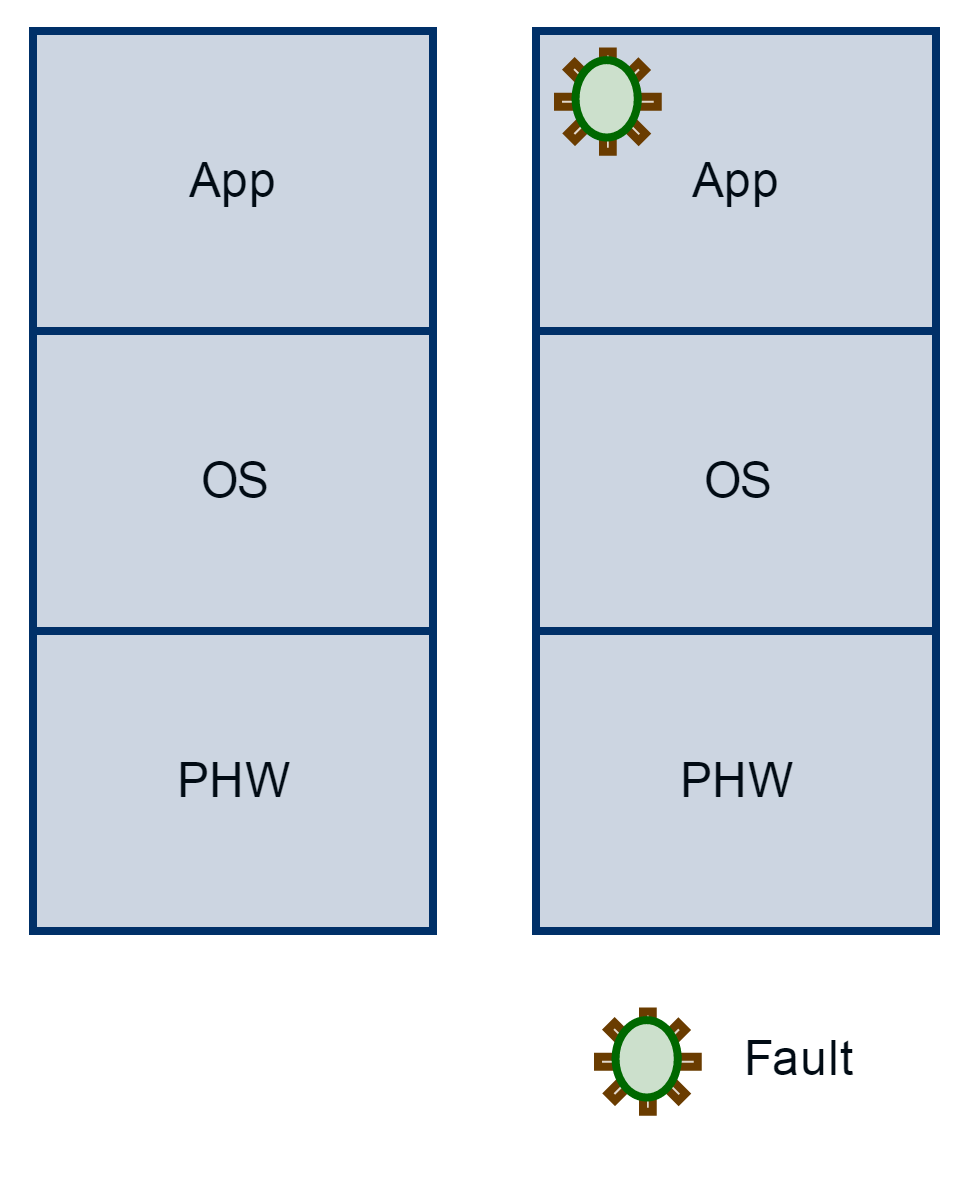
\includegraphics[width=0.4\textwidth]{test1.png}
\caption{\small \sl First and second experiments.\label{fig:test1}}
\end{center}
\end{figure}

The scenario represented in the right of the figure \ref{fig:test1}, it's the same as in the left, with the difference that this have a fault injected in the ``App''. Depending on the type of fault injected into the ``App'', it will have different behaviors, which will be assessed by the \emph{CRASH Scale}.

% \begin{figure}[!ht]
% \begin{center}
% \includegraphics[width=0.2\textwidth]{test2.png}
% \caption{\small \sl Second experiment.\label{fig:test2}}
% \end{center}
% \end{figure}

Above, in the figure \ref{fig:test3}, can be seen the third experiment with an Native Hypervisor. The goal of this scenario is whether through fault injection in one of the virtual machines, the others are affected. And if the virtual machine that don't have faults have the same behavior beside with a execution of a virtual machine with an ``App'' with faults and without faults.

% \begin{figure}[!ht]
% \begin{center}
% 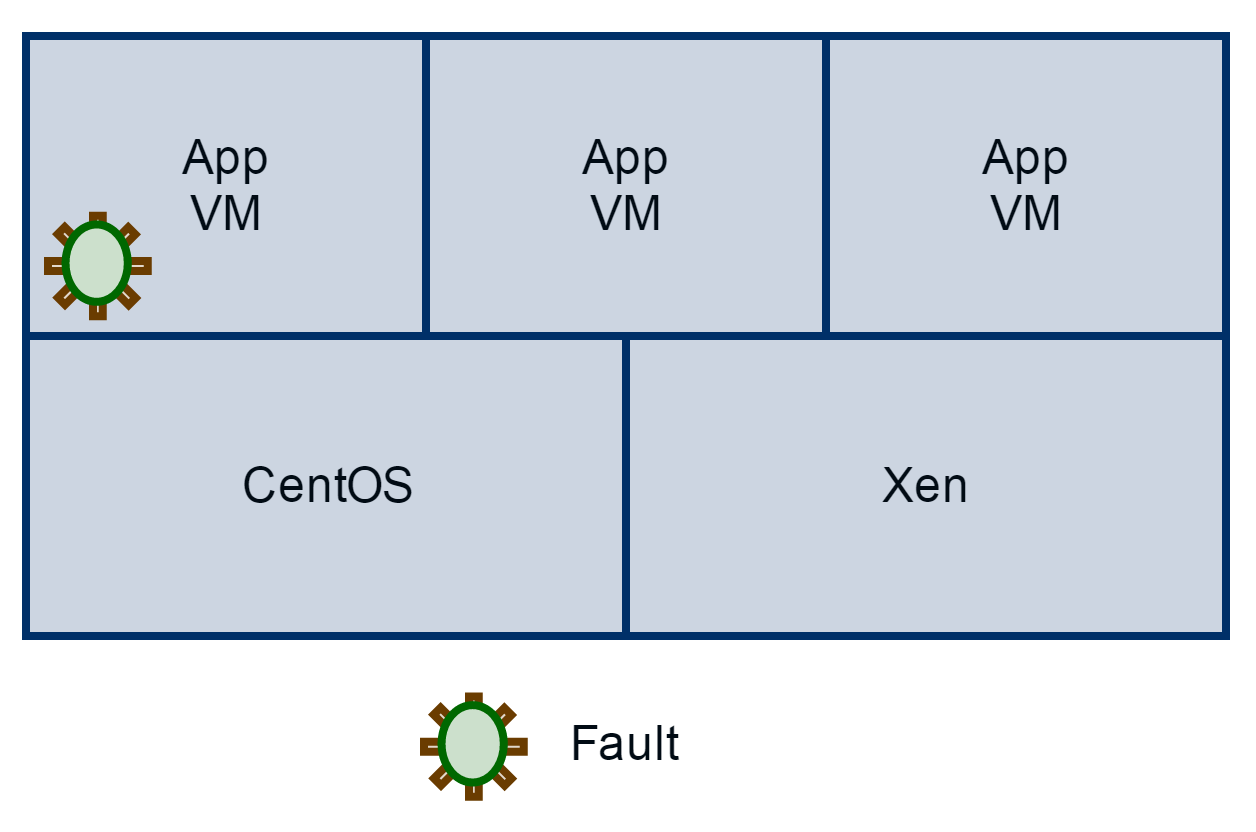
\includegraphics[width=0.5\textwidth]{test3.png}
% \caption{\small \sl Third experiment.\label{fig:test3}}
% \end{center}
% \end{figure}


\begin{figure}[!ht]
\begin{center}
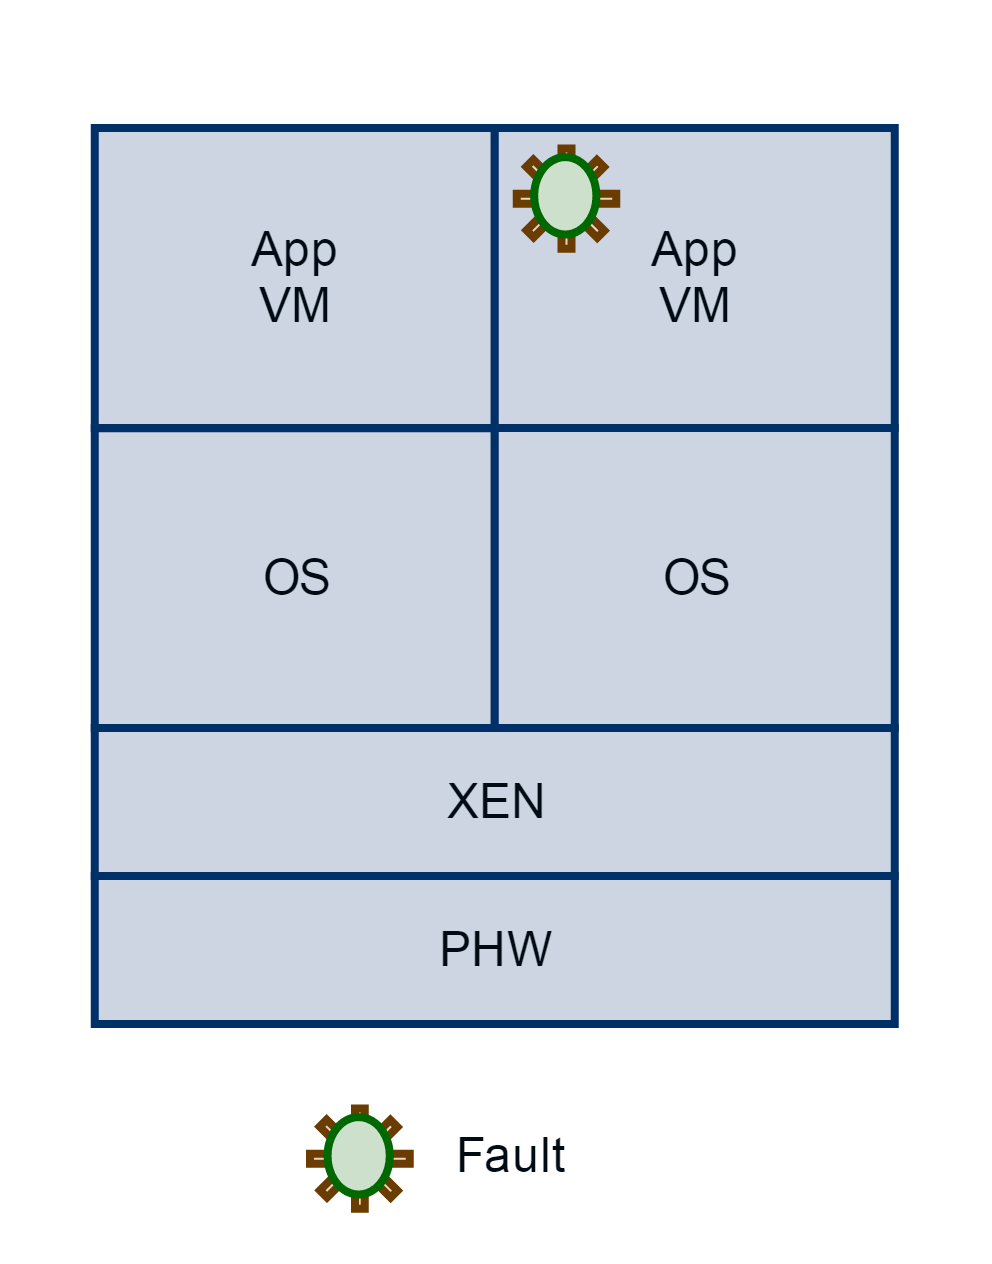
\includegraphics[width=0.4\textwidth]{test4.png}
\caption{\small \sl Third experiment.\label{fig:test3}}
\end{center}
\end{figure}

% \red{The same applications that João Durães has collected information?}
% \begin{itemize}
% 	\item MinGW, Last Update: 2015-06-08
% 	\item ScummVM, Last Update: 2015-05-17
% 	\item CDEX, Last Update: 2015-04-24
% 	\item FireBird, Last Update: 2015-04-15
% 	\item Joe, Last Update: 2015-03-22
% 	\item FreeCiv, Last Update: 2015-03-14
% 	\item GAIM or Pidgin, Last Update: 2015-01-07
% 	\item BASH, Last Update: 2013-12-10
% 	\item ZSNES, Last Update: 2013-05-07
% 	\item VIM, Last Update: 2013-04-25
% 	\item pdftohtml, Last Update: 2013-04-24
% 	%\item LKERNEL
% \end{itemize}

%!TEX root = main.tex

% \newpage


% \vspace*{\fill}
% \begin{center}
	% \section{Appendix}
% \end{center}
% \vspace*{\fill}

\newpage
\appendix
\begin{landscape}
\global\pdfpageattr\expandafter{\the\pdfpageattr/Rotate 90}
\section{Appendix}
\subsection{Gantt diagrams} \label{App:A}

% \begin{figure}[!ht]
% \begin{center}
% \caption{\small \sl First semester gantt.\label{fig:gantt1}}
% \end{center}
% \end{figure}

\begin{figure}[!ht]
\begin{center}
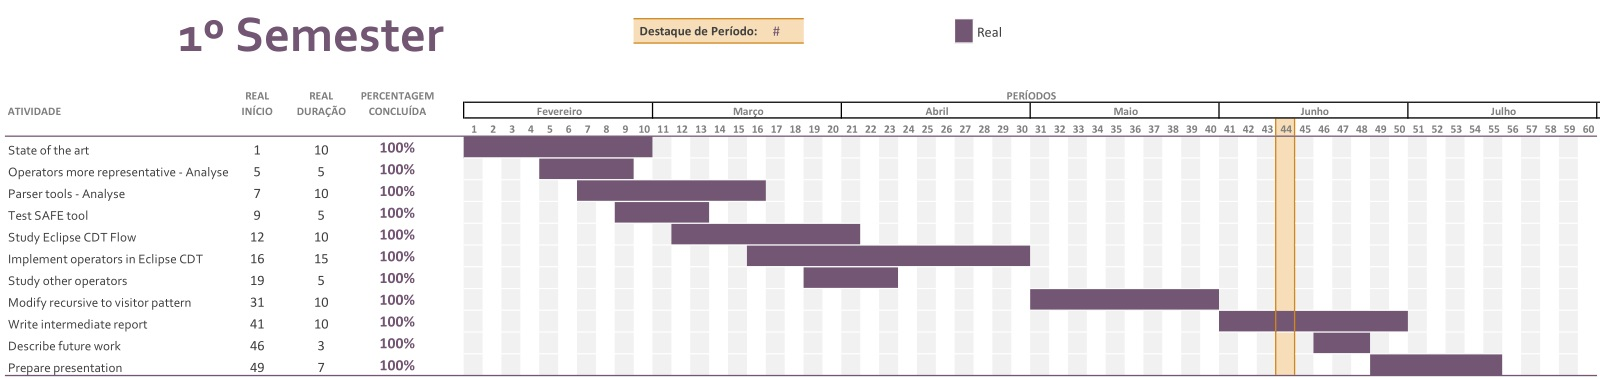
\includegraphics[width=1.6\textwidth]{gantt1.jpg}
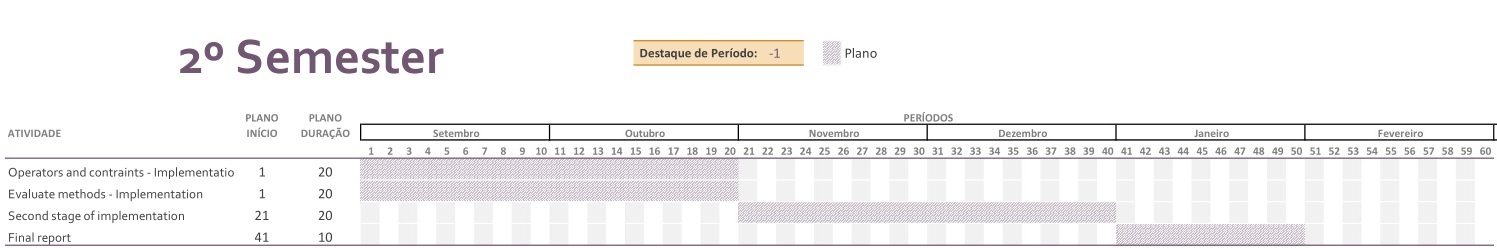
\includegraphics[width=1.6\textwidth]{gantt2.jpg}
\caption{\small \sl First and second semester gantt.\label{fig:gantt}}
\end{center}
\end{figure}

\clearpage

\subsection{Risks table} \label{App:B}
\begin{figure}[!ht]
\begin{center}
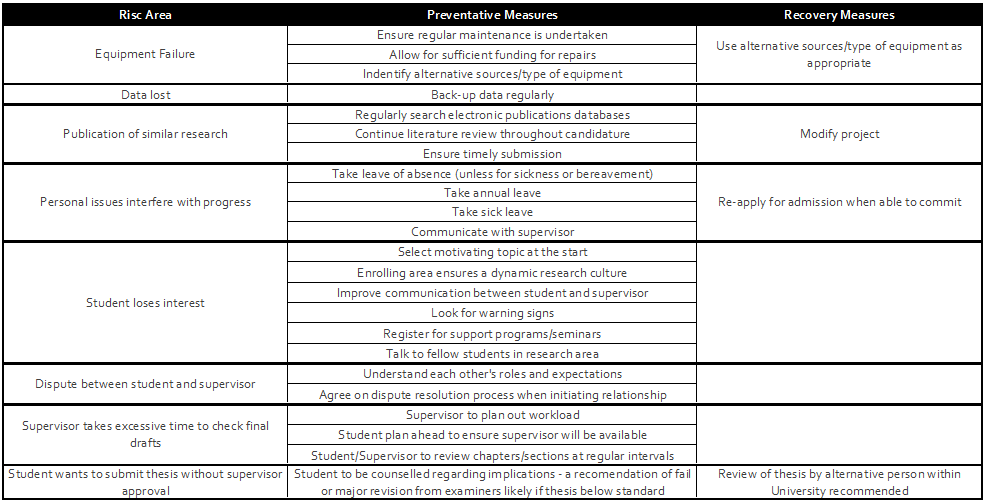
\includegraphics[width=1.5\textwidth]{risks.png}
\caption{\small \sl Risks.\label{fig:risks}}
\end{center}
\end{figure}

\end{landscape}
\global\pdfpageattr\expandafter{\the\pdfpageattr/Rotate 0}

\clearpage
\printacronyms[include-classes=abbrev,name={\subsection{Abbreviations} \label{App:C}}]
% \iftoggle{long}{\acuseall}


% \printacronyms[include-classes=operator,name=Operators]
% \printacronyms[include-classes=constraint,name=Constraints]


% \cleardoublepage
% \phantomsection
% \bibliographystyle{unsrt}
\bibliographystyle{IEEEtran}
\bibliography{refs}
\addcontentsline{toc}{section}{References}
% \nocite{*}

\end{document}
